\documentclass[11pt]{beamer}
\usepackage[utf8]{inputenc}
\usepackage{graphicx, epsfig}
\usepackage{amsmath,mathrsfs,amsfonts,amssymb}
%\usepackage{subfig}
\usepackage{floatflt}
\usepackage{epic,ecltree}
\usepackage{mathtext}
\usepackage{fancybox}
\usepackage{fancyhdr}
\usepackage{multirow}
\usepackage{enumerate}
\usepackage{epstopdf}
\usepackage{multicol}
\usepackage{algorithm}
\usepackage[noend]{algorithmic}
\usepackage{tikz}
\usepackage{blindtext}
\usetheme{default}%{default}%{Singapore}%{Warsaw}%{Warsaw}%{Darmstadt}
\usecolortheme{default}
\setbeamerfont{title}{size=\Huge}
\setbeamertemplate{footline}[page number]{}


\makeatletter
\newcommand\HUGE{\@setfontsize\Huge{35}{40}}
\makeatother    

\setbeamerfont{title}{size=\HUGE}
\beamertemplatenavigationsymbolsempty

% latin bold lower
\newcommand{\ba}{\mathbf{a}} 
\newcommand{\bc}{\mathbf{c}} 
\newcommand{\be}{\mathbf{e}} 
\newcommand{\bh}{\mathbf{h}} 
\newcommand{\bp}{\mathbf{p}} 
\newcommand{\bt}{\mathbf{t}} 
\newcommand{\bs}{\mathbf{s}} 
\newcommand{\bu}{\mathbf{u}} 
\newcommand{\bv}{\mathbf{v}} 
\newcommand{\bw}{\mathbf{w}} 
\newcommand{\bx}{\mathbf{x}} 
\newcommand{\by}{\mathbf{y}} 
\newcommand{\bz}{\mathbf{z}} 

% latin bold upper
\newcommand{\bA}{\mathbf{A}} 
\newcommand{\bB}{\mathbf{B}} 
\newcommand{\bC}{\mathbf{C}} 
\newcommand{\bI}{\mathbf{I}} 
\newcommand{\bL}{\mathbf{L}} 
\newcommand{\bM}{\mathbf{M}} 
\newcommand{\bQ}{\mathbf{Q}} 
\newcommand{\bT}{\mathbf{T}} 
\newcommand{\bU}{\mathbf{U}} 
\newcommand{\bV}{\mathbf{V}} 
\newcommand{\bW}{\mathbf{W}} 
\newcommand{\bX}{\mathbf{X}} 
\newcommand{\bY}{\mathbf{Y}} 
\newcommand{\bZ}{\mathbf{Z}} 

% latin cal upper
\newcommand{\cG}{\mathcal{G}} 
\newcommand{\cL}{\mathcal{L}} 
\newcommand{\cN}{\mathcal{N}} 
\newcommand{\cS}{\mathcal{S}} 
\newcommand{\cT}{\mathcal{T}} 
\newcommand{\cW}{\mathcal{W}} 
\newcommand{\cX}{\mathcal{X}} 
\newcommand{\cZ}{\mathcal{Z}} 

% latin bb upper
\newcommand{\bbE}{\mathbb{E}} 
\newcommand{\bbI}{\mathbb{I}} 
\newcommand{\bbP}{\mathbb{P}} 
\newcommand{\bbR}{\mathbb{R}} 

% greek bold lower
\newcommand{\bepsilon}{\boldsymbol{\epsilon}} 
\newcommand{\btheta}{\boldsymbol{\theta}} 
\newcommand{\blambda}{\boldsymbol{\lambda}} 
\newcommand{\bpi}{\boldsymbol{\pi}} 
\newcommand{\bmu}{\boldsymbol{\mu}} 
\newcommand{\bsigma}{\boldsymbol{\sigma}} 
\newcommand{\bphi}{\boldsymbol{\phi}} 

% greek bold upper
\newcommand{\bSigma}{\boldsymbol{\Sigma}} 

\DeclareMathOperator*{\argmin}{arg\,min}
\DeclareMathOperator*{\argmax}{arg\,max}
\newcommand{\createdgmtitle}[1]{\title[\hbox to 56mm{Mathematical Forecasting Methods \hfill\insertframenumber\,/\,\inserttotalframenumber}]
	{\vspace{1.5\cm} \\ Mathematical Forecasting Methods \\ {\Huge Лекция #1}}
	\author{}
	\institute{
	МФТИ
	} 
	\date{Осень, 2023}
}

\newcommand\myfootnote[1]{%
  \tikz[remember picture,overlay]
  \draw (current page.south west) +(1in + \oddsidemargin,0.5em)
  node[anchor=south west,inner sep=0pt]{\parbox{\textwidth}{%
      \rlap{\rule{10em}{0.4pt}}\raggedright\scriptsize \textit{#1}}};}

\newcommand\myfootnotewithlink[2]{%
  \tikz[remember picture,overlay]
  \draw (current page.south west) +(1in + \oddsidemargin,0.5em)
  node[anchor=south west,inner sep=0pt]{\parbox{\textwidth}{%
      \rlap{\rule{10em}{0.4pt}}\raggedright\scriptsize\href{#1}{\textit{#2}}}};}
\createdgmtitle{7}
\usepackage{tikz}
\usepackage{amsmath}
\usepackage[english,russian]{babel}
\usepackage[labelformat=empty]{caption}

\usepackage{graphicx,animate}
\usepackage{animate}
\usepackage{svg}
\usepackage{subcaption}

\usetikzlibrary{arrows,shapes,positioning,shadows,trees}
\newcommand*{\defeq}{\stackrel{\text{def}}{=}}

%--------------------------------------------------------------------------------
\begin{document}
%--------------------------------------------------------------------------------
\begin{frame}[plain]
%\thispagestyle{empty}
\titlepage
\end{frame}
%=======
\begin{frame}{Краткое повторение}
\begin{itemize}
    \item Вектор задержек и матрица задержек -- это удобные способы многомерного представления временного ряда.
    \item Метод SSA основан на сингулярном разложении матрицы задержек ряда.
    \item Низкоранговое приближение позволяет осуществить SSA-сглаживание временного ряда, что помогает уменьшить влияние шума.
\end{itemize}
\end{frame}
%=======

\begin{frame}{Матричное представление временного ряда}
\begin{itemize}
    \item Вектор задержек: 
    $$ \mathbf{x}_t = (x_t, x_{t+1}, \dots, x_{t + \tau - 1})^T \in \mathbb{R}^{\tau}$$
    \item Матрица задержек:
    $$\mathbf{X} = 
    \begin{pmatrix}
    \mathbf{x}_1 & \mathbf{x}_2 & \mathbf{x}_3 & \dots & \mathbf{x}_{\tau} & \dots & \mathbf{x}_n
    \end{pmatrix} = $$
    $$ = \begin{pmatrix}
    x_1 & x_2 & x_3 & \dots & x_{\tau} & \dots & x_n \\
    x_2 & x_3 & x_4 & \dots & x_{\tau + 1} & \dots & x_{n + 1} \\
    x_3 & x_4 & x_5 & \dots & x_{\tau + 2} & \dots & x_{n + 2} \\
    \vdots & \vdots & \vdots & \ddots & \vdots & \ddots & \vdots \\
    x_{\tau} & x_{\tau + 1} & x_{\tau + 2} & \dots & x_{2\tau - 1} & \dots & x_N 
    \end{pmatrix} \in \mathbb{R}^{\tau \times n}$$
    Здесь предполагаем, что $n > \tau$.
\end{itemize}
\end{frame}
%=======
\begin{frame}{SVD: напоминание}
    Для матрицы $\mathbf{X}$ существует (и, вообще говоря, не единственно) сингулярное разложение:
    $$ \underset{\tau \times n}{\mathbf{X}} = \underset{\tau \times \tau}{\text{U}} \ \underset{\tau \times n}{\Sigma} \ \underset{n \times n}{V^T}$$
    Здесь:
    \begin{itemize}
        \item $\text{U} \in \mathbb{R}^{\tau \times \tau}$ -- ортогональная матрица собств. векторов $\mathbf{X}\mathbf{X}^T$ (столбцы $\text{U}$ образуют ортонормированный базис в $\mathbb{R}^{\tau}$)
        \item $\Sigma \in \mathbb{R}^{\tau \times n}$ -- прямоугольная диагональная матрица сингулярных чисел $\mathbf{X}$, причем $\sigma_1 \geq \sigma_2 \geq \dots \geq \sigma_{\tau}$:
        $$ \Sigma = \begin{pmatrix}
            \sigma_1  & \dots & 0 & 0 & \dots & 0 \\
            \vdots  & \ddots & \vdots & \vdots & \dots & \vdots \\
            0 &  \dots & \sigma_{\tau} & 0 & \dots & 0
        \end{pmatrix}$$
        \item $V \in \mathbb{R}^{n \times n}$ -- ортогональная матрица собств. векторов $\mathbf{X}^T\mathbf{X}$ (столбцы $V$ образуют ортонормированный базис в $\mathbb{R}^{n}$)
    \end{itemize}
\end{frame}
%=======
\begin{frame}{Low Rank Approximation}
    Одним из важных свойств сингулярного разложения матрицы является возможность построения для неё \textit{низкорангового приближения}, а именно:
    \begin{itemize}
        \item Пусть $A \in \mathbb{R}^{m \times n}$, $ A = \text{U} \Sigma V^T$ -- сингулярное разложение $A$.
        \item Рассмотрим матрицу $\Sigma$ и её приближение ранга $r$ -- матрицу $\tilde{\Sigma}$, где подматрица $\Sigma_1$ имеет размер $r \times r$:
        $$ \Sigma = 
        \begin{bmatrix}
        \Sigma_1 & 0 \\
        0 & \Sigma_2
        \end{bmatrix}, \quad 
        \tilde{\Sigma} = 
        \begin{bmatrix}
        \Sigma_1 & 0 \\
        0 & 0
        \end{bmatrix}$$
        \item \textbf{Теорема:} среди всех матриц $B$ ранга не более $r$ норма разности матриц $A$ и $\tilde{A} = \text{U} \tilde{\Sigma} V^T$ минимальна: 
        $$\tilde{A} = \argmin_{\text{rank}(B) \leq r}{|| A - B ||} \quad \text{(верно для $|| \cdot ||_2$, для $|| \cdot ||_F$)}$$
        
        \item Матрица $\tilde{A}$ также может быть получена, как $\tilde{A} = \text{U}_1 \Sigma_1 V_1^T$, где $\text{U}_1, \ V_1$ -- первые $r$ столбцов матриц $\text{U}$ и $V$.
        
    \end{itemize}
\end{frame}
%=======

\begin{frame}{Прогноз в методе SSA}
    Пусть нам известны значения временного ряда $x_1, ..., x_N$, и ряд представлен в виде матрицы задержек $\mathbf{X} = (\mathbf{x}_1, ..., \mathbf{x}_{N - \tau + 1})$. Следующему, неизвестному, значению ряда $x_{N+1}$ сопоставим вектор задержек $\mathbf{x}_{N - \tau + 2}$:
    $$ \mathbf{X} = \begin{pmatrix}
    x_1 &  \dots & x_{N - \tau + 1} \\
    x_2 &  \dots & x_{N - \tau + 2} \\
    \vdots &  \ddots & \vdots \\
    x_{\tau} & \dots & x_N 
    \end{pmatrix}, \quad 
    \mathbf{x}_{N - \tau + 2} = \begin{pmatrix}
        x_{N - \tau + 2} \\
        x_{N - \tau + 3} \\
        \vdots \\
        x_{N  + 1} \\
    \end{pmatrix} $$

    Для матрицы $\mathbf{X}$ построим низкоранговое приближение $\tilde{\mathbf{X}} = \text{U}_1 \Sigma_1 V_1^T$, где 
    
    $$\text{U}_1 = \Big(\mathbf{u}_1, ..., \mathbf{u}_r\Big) = 
    \begin{pmatrix}
    u^{(1)}_1 & \dots & u^{(r)}_1 \\
    \vdots & \ddots & \vdots \\
    u^{(1)}_\tau & \dots & u^{(r)}_\tau 
    \end{pmatrix} \in \mathbb{R}^{\tau \times r}$$
    -- матрица базисных векторов $r$-мерного подпространства в $\mathbb{R}^{\tau}$.
\end{frame}
%=======


\begin{frame}{Восстановление неизвестных компонент вектора}
\textbf{Определение.} \textit{Ограничением} вектора $\mathbf{x} = (x_1, ..., x_\tau)^T \in \mathbb{R}^\tau$ на множество индексов $\mathcal{P} = \{ i_1, ..., i_{|\mathcal{P}|}\} \subset \mathcal{I} = \overline{1,\tau}$ называется вектор $\mathbf{x}\vert_{\mathcal{P}} = (x_{i_1}, ..., x_{i_{|\mathcal{P}|}})^T \in \mathbb{R}^{|\mathcal{P}|}$. Аналогично можно определить ограничение матрицы $\text{A}$ и ограничение линейного подпространства $\mathcal{L}$ (обозначаются, соответственно, $\text{A}\vert_{\mathcal{P}}$ и $\mathcal{L}\vert_{\mathcal{P}}$). \\

\vspace{0.3cm}
\newline
Рассмотрим линейное подпространство $\mathcal{L}_r$ евклидова пространства $\mathbb{R}^\tau$. Пусть его ортонормированный базис $\mathbf{u}_1, ..., \mathbf{u}_r$ образует матрицу $\text{U} = [\mathbf{u}_1, ..., \mathbf{u}_r] \in \mathbb{R}^{\tau \times r}$. Пусть зафиксировано множество индексов $\mathcal{P}$.\\
\textbf{Теорема.} Пусть матрица $\text{I}_{|\mathcal{P}|} - \text{U}\vert_{\mathcal{P}} \text{U}\vert_{\mathcal{P}}^T$ обратима. Тогда для любого вектора $\mathbf{x} \in \mathcal{L}_r$ компоненты ограничения $\mathbf{x}\vert_{\mathcal{P}}$ выразимы через остальные компоненты $\mathbf{x}\vert_{\mathcal{I} \textbackslash \mathcal{P}}$:

$$ \mathbf{x}\vert_{\mathcal{P}} = \Big( \text{I}_{|\mathcal{P}|} - \text{U}\vert_{\mathcal{P}} \text{U}\vert_{\mathcal{P}}^T \Big)^{-1} \text{U}\vert_{\mathcal{P}} \text{U}\vert_{\mathcal{I} \textbackslash \mathcal{P}}^T \mathbf{x}\vert_{\mathcal{I} \textbackslash \mathcal{P}}$$

\textbf{Замечание.} Обратимость матрицы из условия теоремы эквивалентна равенству рангов матриц $\text{U}$ и $\text{U}\vert_{\mathcal{I} \textbackslash \mathcal{P}}$.

\end{frame}
%=======

\begin{frame}{Доказательство теоремы }
    \begin{enumerate}
        \item Без ограничения общности пусть $\mathcal{P} = \{1, ..., |\mathcal{P}| \}$.
        \item Обозначим $\mathbf{x}_1 = \mathbf{x}\vert_{\mathcal{P}}, \mathbf{x}_2 = \mathbf{x}\vert_{\mathcal{I} \textbackslash \mathcal{P}}, \text{U}_1 = \text{U}\vert_{\mathcal{P}}, \text{U}_2 = \text{U}\vert_{\mathcal{I} \textbackslash \mathcal{P}}$.
        \item Для любого $\mathbf{x} \in \mathcal{L}_r$ верно, что $\text{U}\text{U}^T\mathbf{x} = \mathbf{x}$. При этом произведение $\text{U}\text{U}^T$ можно представить в следующем блочном виде:
        $$ \text{U}\text{U}^T = \begin{bmatrix}
            \text{U}_1\text{U}_1^T & \text{U}_1 \text{U}_2^T \\
            \vspace{0.05cm}\\
            \text{U}_2 \text{U}_1^T & \text{U}_2 \text{U}_2^T
        \end{bmatrix}$$
        Тогда справедливо равенство $\mathbf{x}_1 = \text{U}_1\text{U}_1^T\mathbf{x}_1 + \text{U}_1 \text{U}_2^T \mathbf{x}_2$.
        \item Отсюда получаем равенство: 
        $$\Big(\text{I}_{|\mathcal{P}|} - \text{U}_1\text{U}_1^T\Big)\mathbf{x}_1 = \text{U}_1 \text{U}_2^T \mathbf{x}_2$$
        Остаётся лишь домножить обе части равенства на обратную матрицу и перейти к исходным обозначениям.
    \end{enumerate}
        

\end{frame}

%=======


\begin{frame}{Прогноз в методе SSA (упрощённый вариант)}
    В качестве индексного множества выберем $\mathcal{P} = \{ \tau \}$.\\ 
    В качестве $\mathbf{x}$ возьмём $\mathbf{x}_{N - \tau + 2}$. Тогда:
    \begin{itemize}
        \item $\mathbf{x}\vert_{\mathcal{P}} = x_{N+1}$
        \item $\mathbf{x}\vert_{\mathcal{I} \textbackslash \mathcal{P}} = \big( x_{N - \tau + 2}, x_{N - \tau + 3}, \dots, x_N\big)^T$
    \end{itemize}
    Предположим, что $\mathbf{x}$ лежит в линейном подпространстве с базисом $\text{U} := \text{U}_1$ (упрощение).
    Тогда:\\
    \vspace{0.3cm}
    \begin{itemize}
        \item $\text{U}\vert_{\mathcal{P}} = \Big(u^{(1)}_\tau & \dots & u^{(r)}_\tau \Big)$
        \item $\text{I}_{|\mathcal{P}|} - \text{U}\vert_{\mathcal{P}} \text{U}\vert_{\mathcal{P}}^T = 1 - \displaystyle \sum_{i=1}^r \Big(u^{(i)}_\tau \Big)^2$
        \item $ \text{U}\vert_{\mathcal{I} \textbackslash \mathcal{P}} = \begin{pmatrix}
    u^{(1)}_1 & \dots & u^{(r)}_1 \\
    \vdots & \ddots & \vdots \\
    u^{(1)}_{\tau - 1} & \dots & u^{(r)}_{\tau - 1} 
    \end{pmatrix} \in \mathbb{R}^{(\tau - 1) \times r}$
    \end{itemize}
    
    
\end{frame}
%=======

\begin{frame}{Прогноз в методе SSA (упрощённый вариант)}
    Окончательно, пользуясь теоремой, восстанавливаем неизвестное значение:

    $$ x_{N+1} = \frac{1}{1 - \displaystyle \sum_{i=1}^r \Big(u^{(i)}_\tau \Big)^2} \text{U}\vert_{\mathcal{P}} \text{U}\vert_{\mathcal{I} \textbackslash \mathcal{P}}^T \mathbf{x}\vert_{\mathcal{I} \textbackslash \mathcal{P}}$$

    Прогноз на несколько шагов вперёд рассчитывается последовательным построением прогноза на один шаг вперёд, при этом можно либо каждый раз перестраивать матрицу задержек $\mathbf{X}$, её сингулярное разложение и низкоранговое приближение, либо оперировать одной и той же матрицей $\mathbf{X}$ (а значит, той же матрицей $\text{U}$) для построения последовательных прогнозов.
    
\end{frame}



\begin{frame}{Проблема сравнения двух последовательностей}
Поэлементное сравнение временных рядов в терминах, например, евклидового расстояния не является адекватной мерой близости рядов в случае, когда второй ряд получен в результате смещения первого.
\begin{figure}
    \centering
    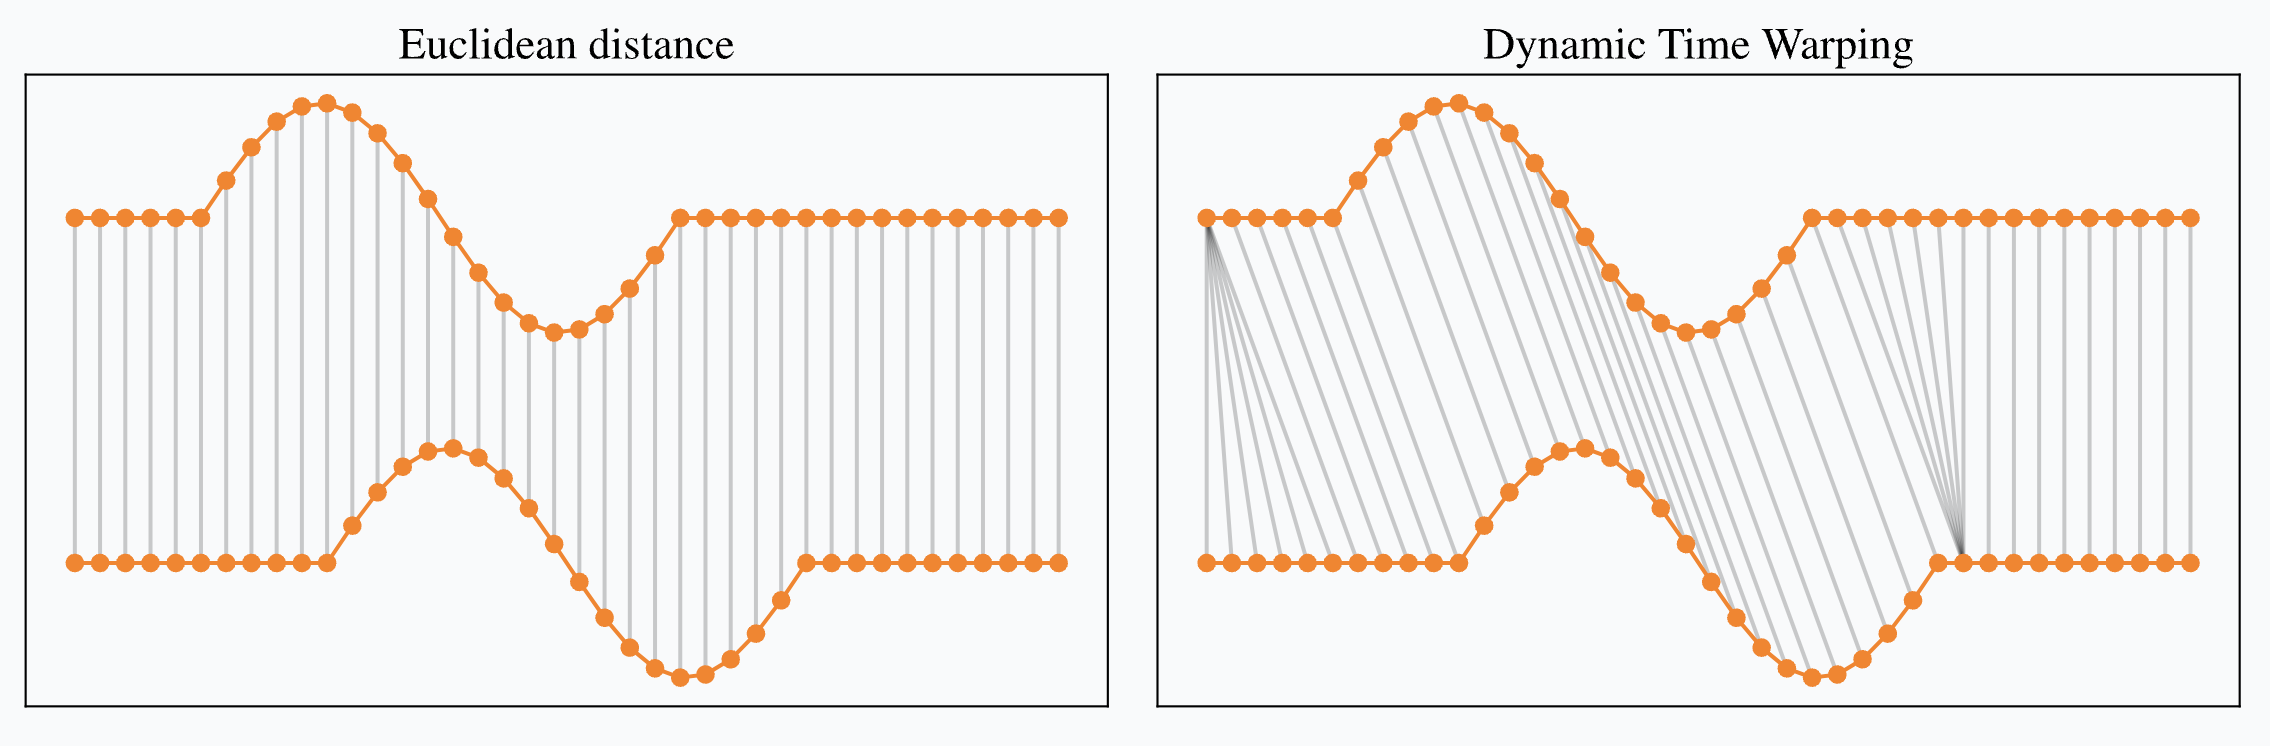
\includegraphics[width=\textwidth]{lecture_7/figs/dtw_vs_euc.png}
\end{figure}
\myfootnotewithlink{https://rtavenar.github.io/blog/dtw.html#dynamic-time-warping}{сredit: https://rtavenar.github.io/blog/dtw.html#dynamic-time-warping}
\end{frame}
%=======
%=======
\begin{frame}{Проблема вычисления среднего}
\begin{figure}
    \centering
    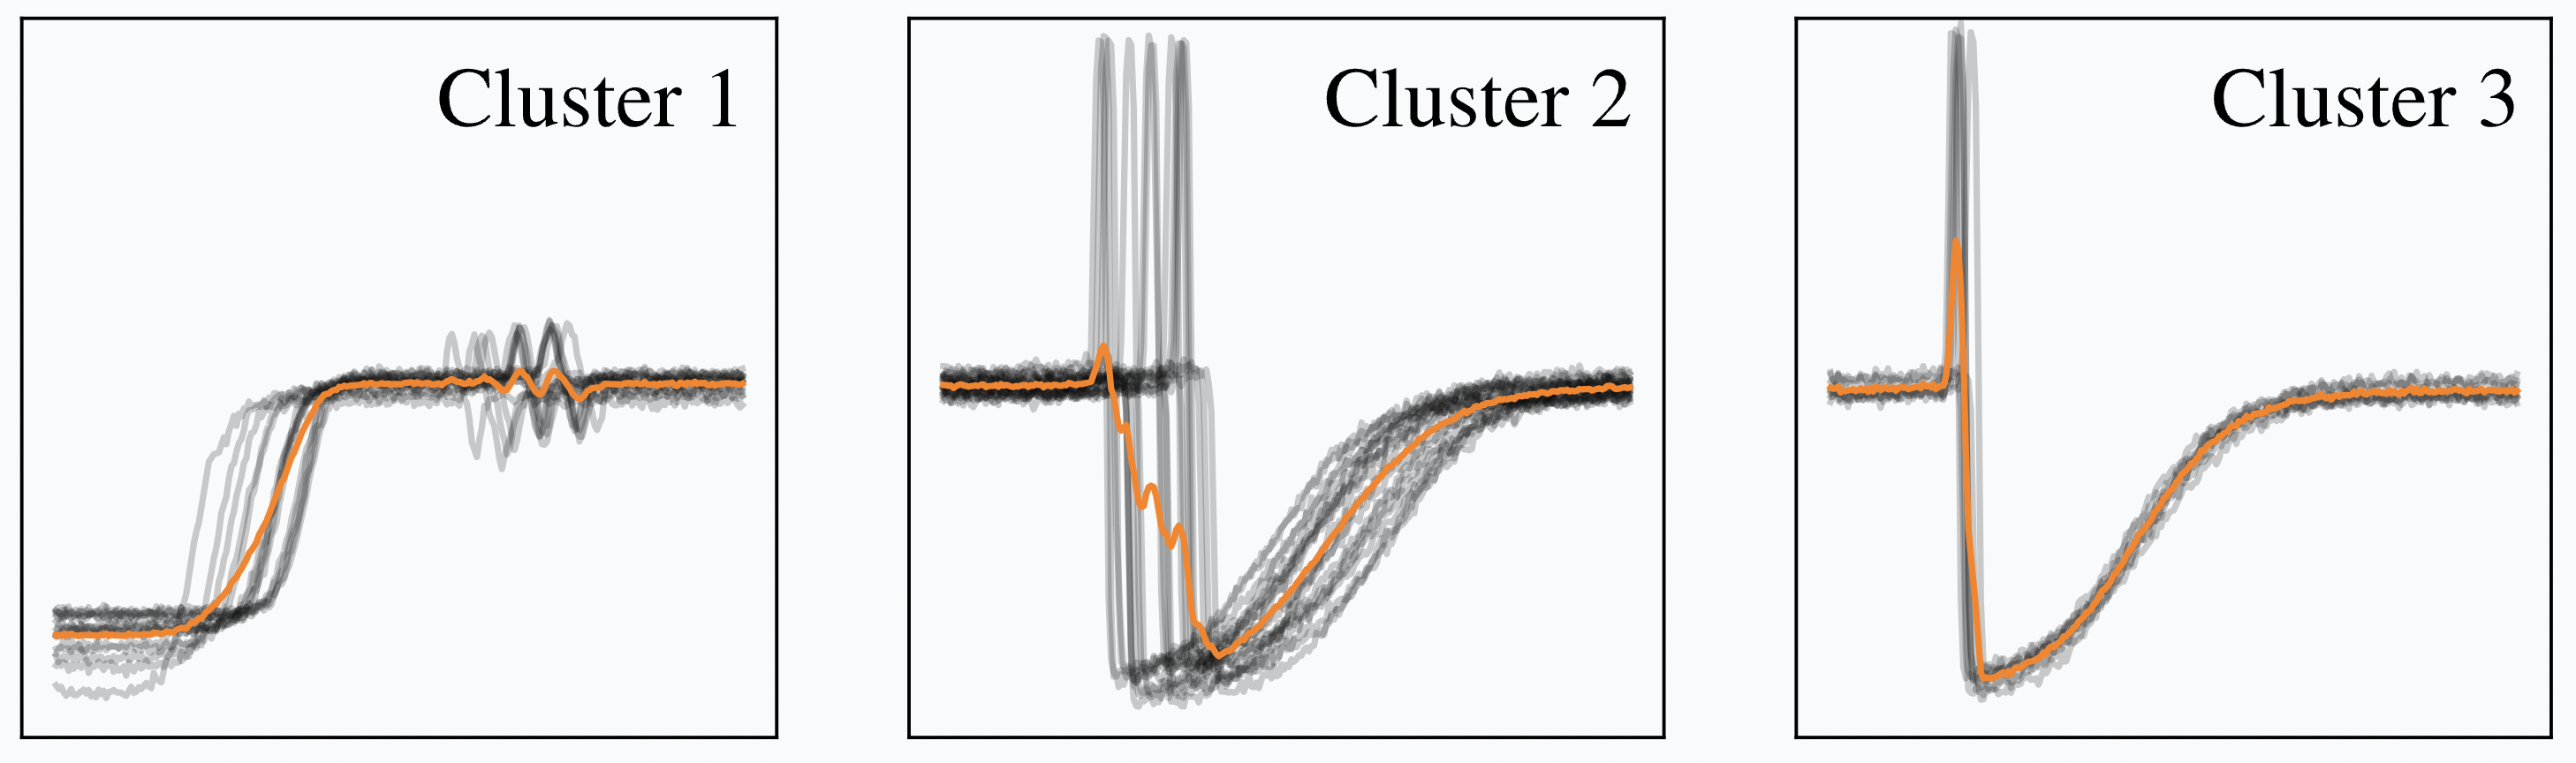
\includegraphics[width=\textwidth]{lecture_7/figs/cluster_1.png}
    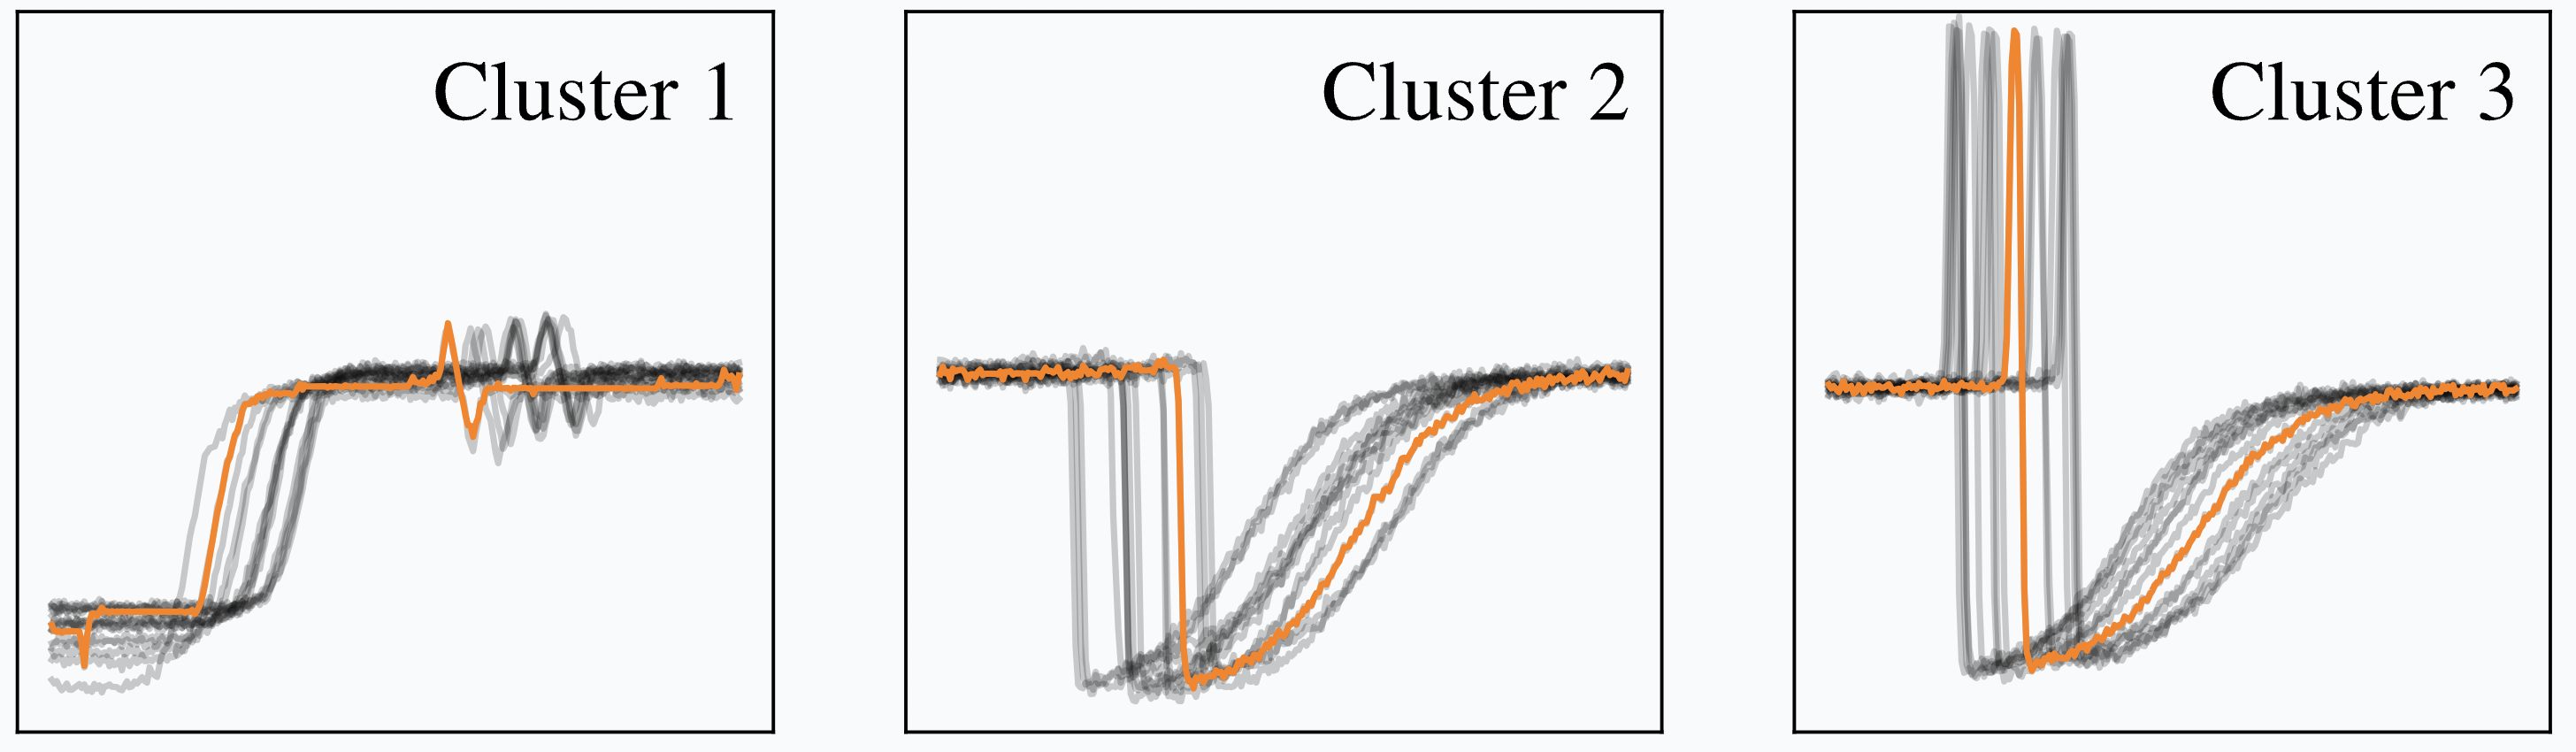
\includegraphics[width=\textwidth]{lecture_7/figs/cluster_2.png}
    \caption{Сверху: кластеры, полученные алгоритмом K-means ($K = 3$), метрика - поэлементная сумма евклидовых расстояний. \\
    Снизу: аналогичные кластеры, функция расстояния - DTW}
\end{figure}
\end{frame}

\begin{frame}{Dynamic time warping}

\textbf{Dynamic time warping} (\textit{DTW, Динамическое искажение времени}) -- функция расстояния, позволяющая оценивать поэлементную близость временных рядов \textit{с точностью до сдвига/растяжения во времени}.\\
\vspace{0.2cm}

Рассмотрим два временных ряда $x$ и $x'$, возможно, различной длины $n$ и $m$. Тогда DTW определяется следующим образом:

$$ DTW_q( x, x^{'}) = \min_{\pi \in \mathcal{A}(x, x^{'})}\Bigg( \sum_{(i,j) \in \pi} d(x_i, x_j^{'})^q \Bigg).$$

Здесь $\pi$ -- \textit{временное выравнивание}, т.е. последовательность пар индексов $\big( (i_0, j_0), \dots, (i_{K-1}, j_{K-1})  \big)$ длины $K = K(\pi)$ из семейства всевозможных допустимых выравниваний $\mathcal{A}(x, x^{'})$. 

\end{frame}
%=======

\begin{frame}{Допустимое выравнивание временных рядов}
    Выравнивание является допустимым, если:
\begin{enumerate}
    \item Начало и конец обеих временных рядов сопоставлены друг другу в качестве первой и последней пары выравнивания:\\
    \vspace{0.2cm}
    $\quad \displaystyle \pi_0 = (0, 0)$\\
    $\quad \displaystyle \pi_K = (n-1, m-1)$


    \item Последовательность пар индексов монотонно не убывает по обеим компонентам, и каждое значение индексов обеих временных рядов встречается в последовательности хотя бы 1 раз:\\
    \vspace{0.2cm}
    $\quad \displaystyle i_{k-1} \leq i_k \leq i_{k-1} + 1$\\
    $\quad \displaystyle j_{k-1} \leq j_k \leq j_{k-1} + 1$

\end{enumerate}
\end{frame}

%=======
\begin{frame}{Dynamic time warping, иллюстрация}
\begin{figure}
    \centering
    \animategraphics[autoplay,loop,width=0.8\textwidth]{10}{lecture_7/figs/gif_1/000}{6}{45}
\end{figure}

\end{frame}

%=======
\begin{frame}{Матричное представление допустимого выравнивания}
Допустимому выравниванию $\pi$ можно сопоставить матрицу:
$$ \big(A_\pi \big)_{i,j} = \begin{cases}
    1, \text{ если } (i,j) \in \pi \\
    0, \text{ иначе }
\end{cases}$$
Всевозможные допустимые выравнивания соответствуют всевозможным \textit{правильным путям} в матрице размера $n \times m$ из левого верхнего угла в правый нижний.
\begin{figure}
    \centering
    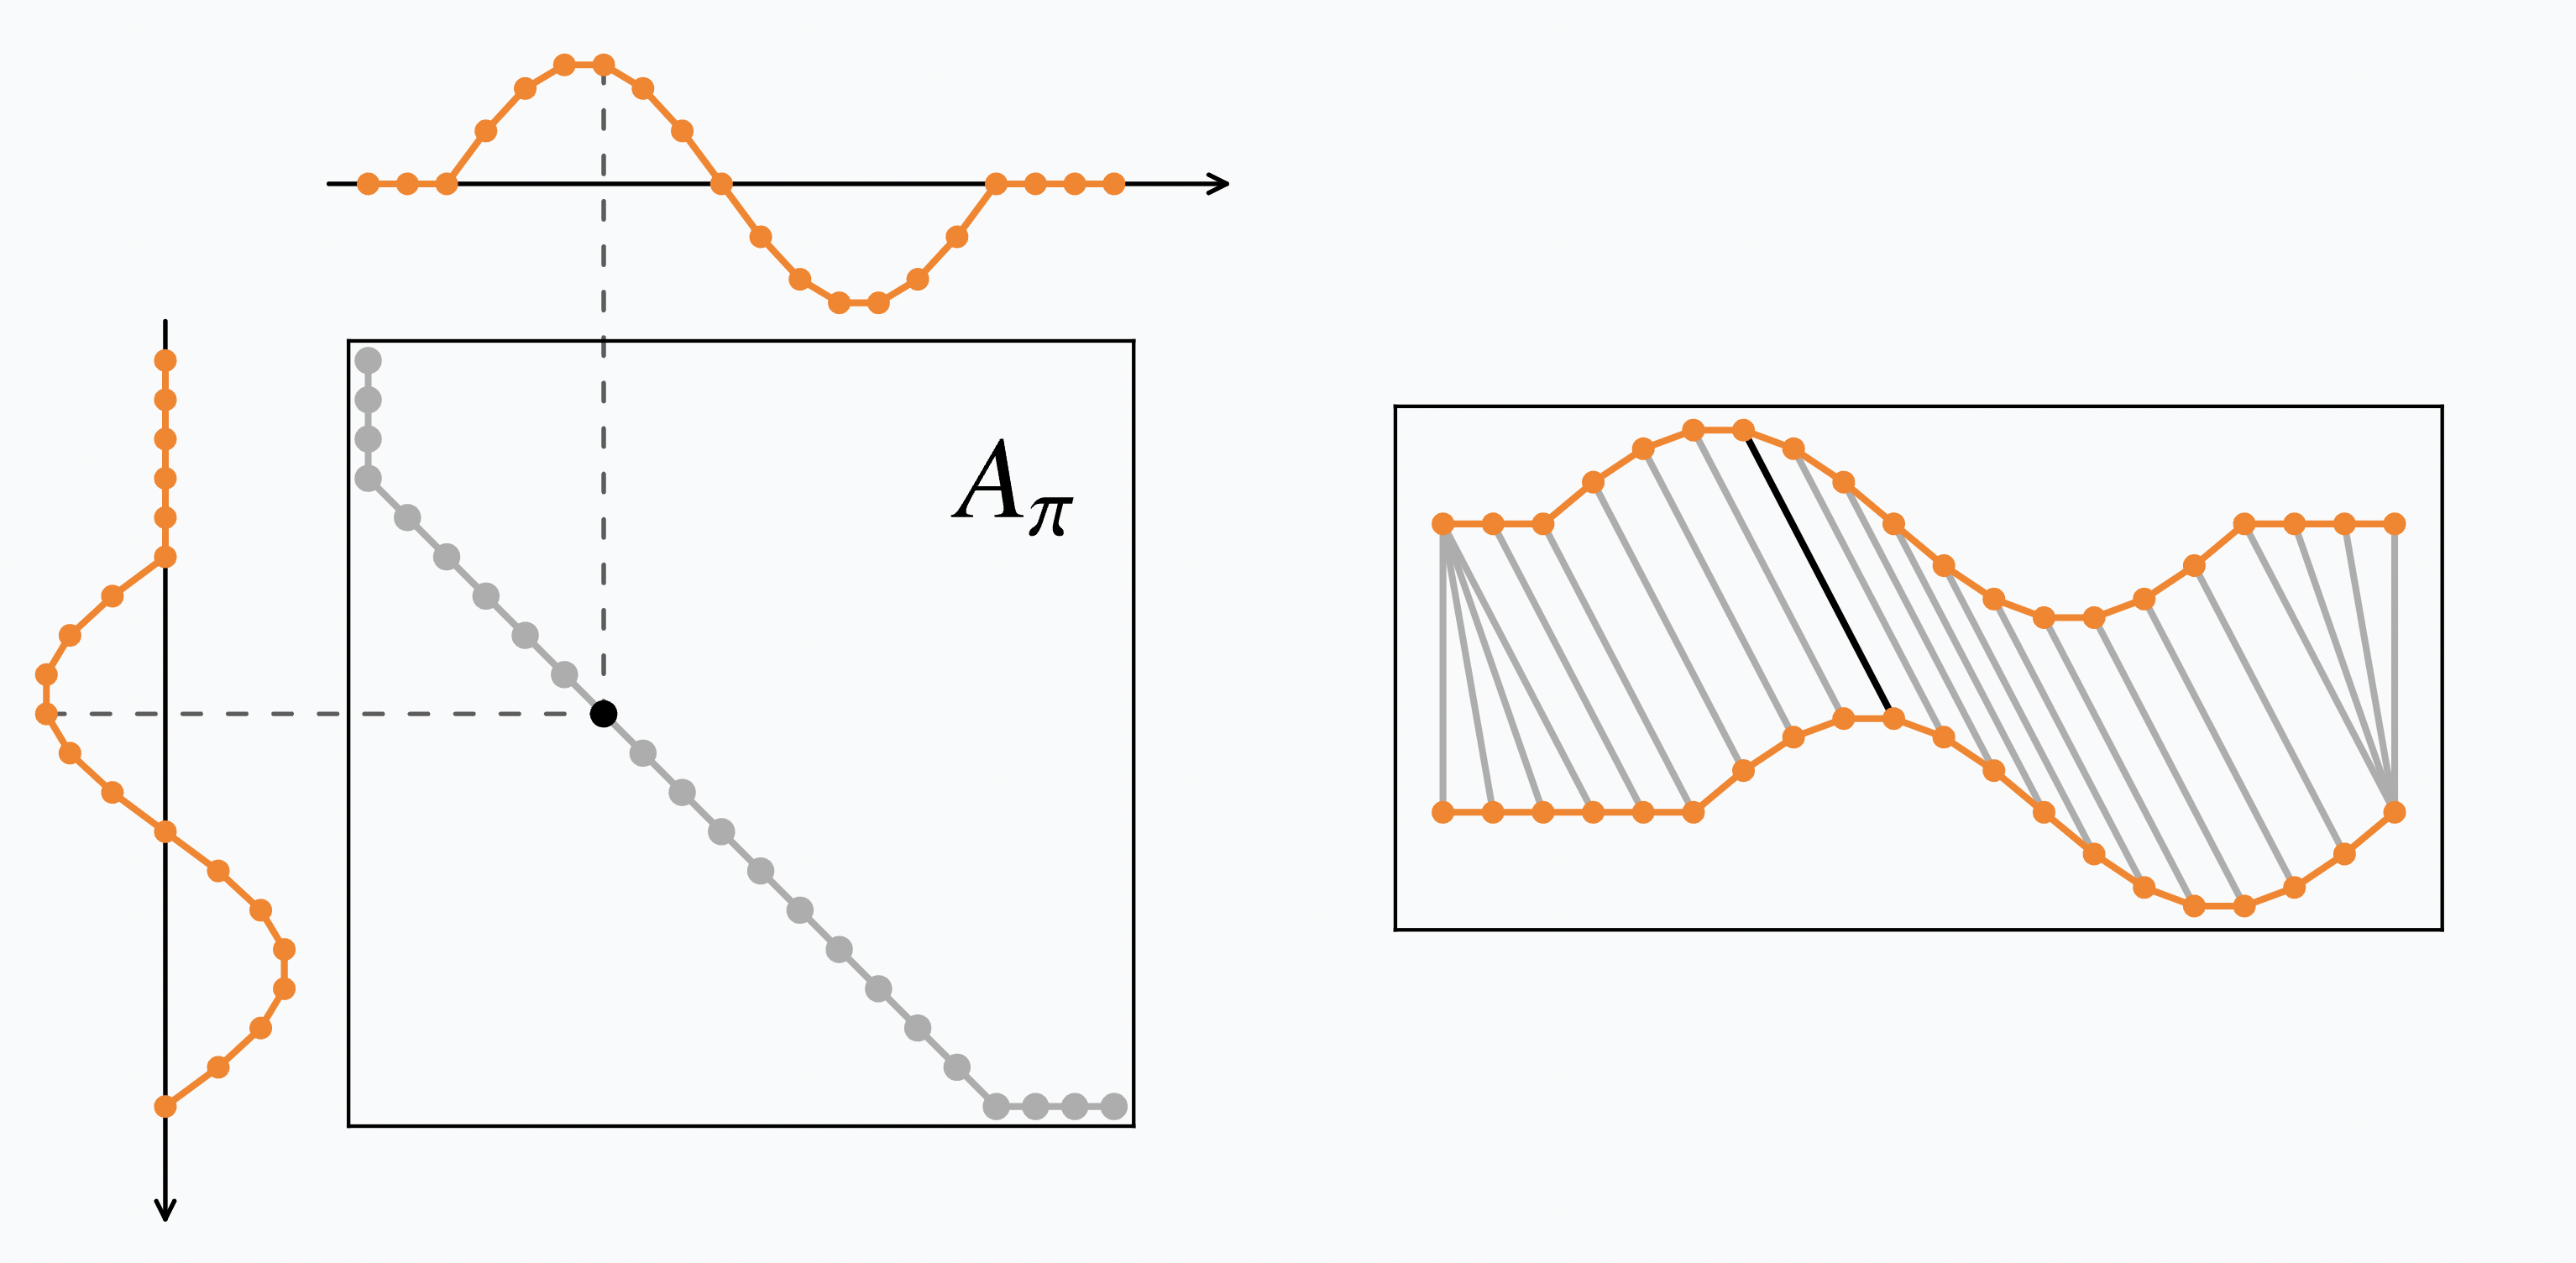
\includegraphics[width=0.8\textwidth]{lecture_7/figs/matrix_1.png}
\end{figure}
\end{frame}

%=======

\begin{frame}{Динамическое программирование для нахождения DTW}

Нахождение DTW в лоб приводит к экспоненциальному перебору по всевозможным допустимым путям, но существует эффективный алгоритм для расчёта DTW с помощью динамического программирования. \\
Идея: можно рассчитывать промежуточные значения DTW для коротких отрезков исходных временных рядов
 $$ R_{i,j} = DTW_q( x_{\rightarrow i}, x_{\rightarrow j}^{'}),$$
а потом заметить рекуррентную связь:

$$ R_{i,j}  = \min_{\pi \in \mathcal{A}(x_{\rightarrow i}, x_{\rightarrow j}^{'})}\Bigg( \sum_{(k,l) \in \pi} d(x_k, x_l^{'})^q \Bigg) $$

$$ = d(x_i, x_j^{'})^q +  \min_{\pi \in \mathcal{A}(x_{\rightarrow i}, x_{\rightarrow j}^{'})}\Bigg( \sum_{(k,l) \in \pi[:-1]} d(x_k, x_l^{'})^q \Bigg)$$
$$ = d(x_i, x_j^{'})^q  + \min(\textcolor{blue}{R_{i-1, j}}, \textcolor{red}{R_{i,j-1}}, \textcolor{green}{R_{i-1,j-1}})$$

\end{frame}
%=======

\begin{frame}{Динамическое программирование для нахождения DTW}
\begin{figure}
    \centering
    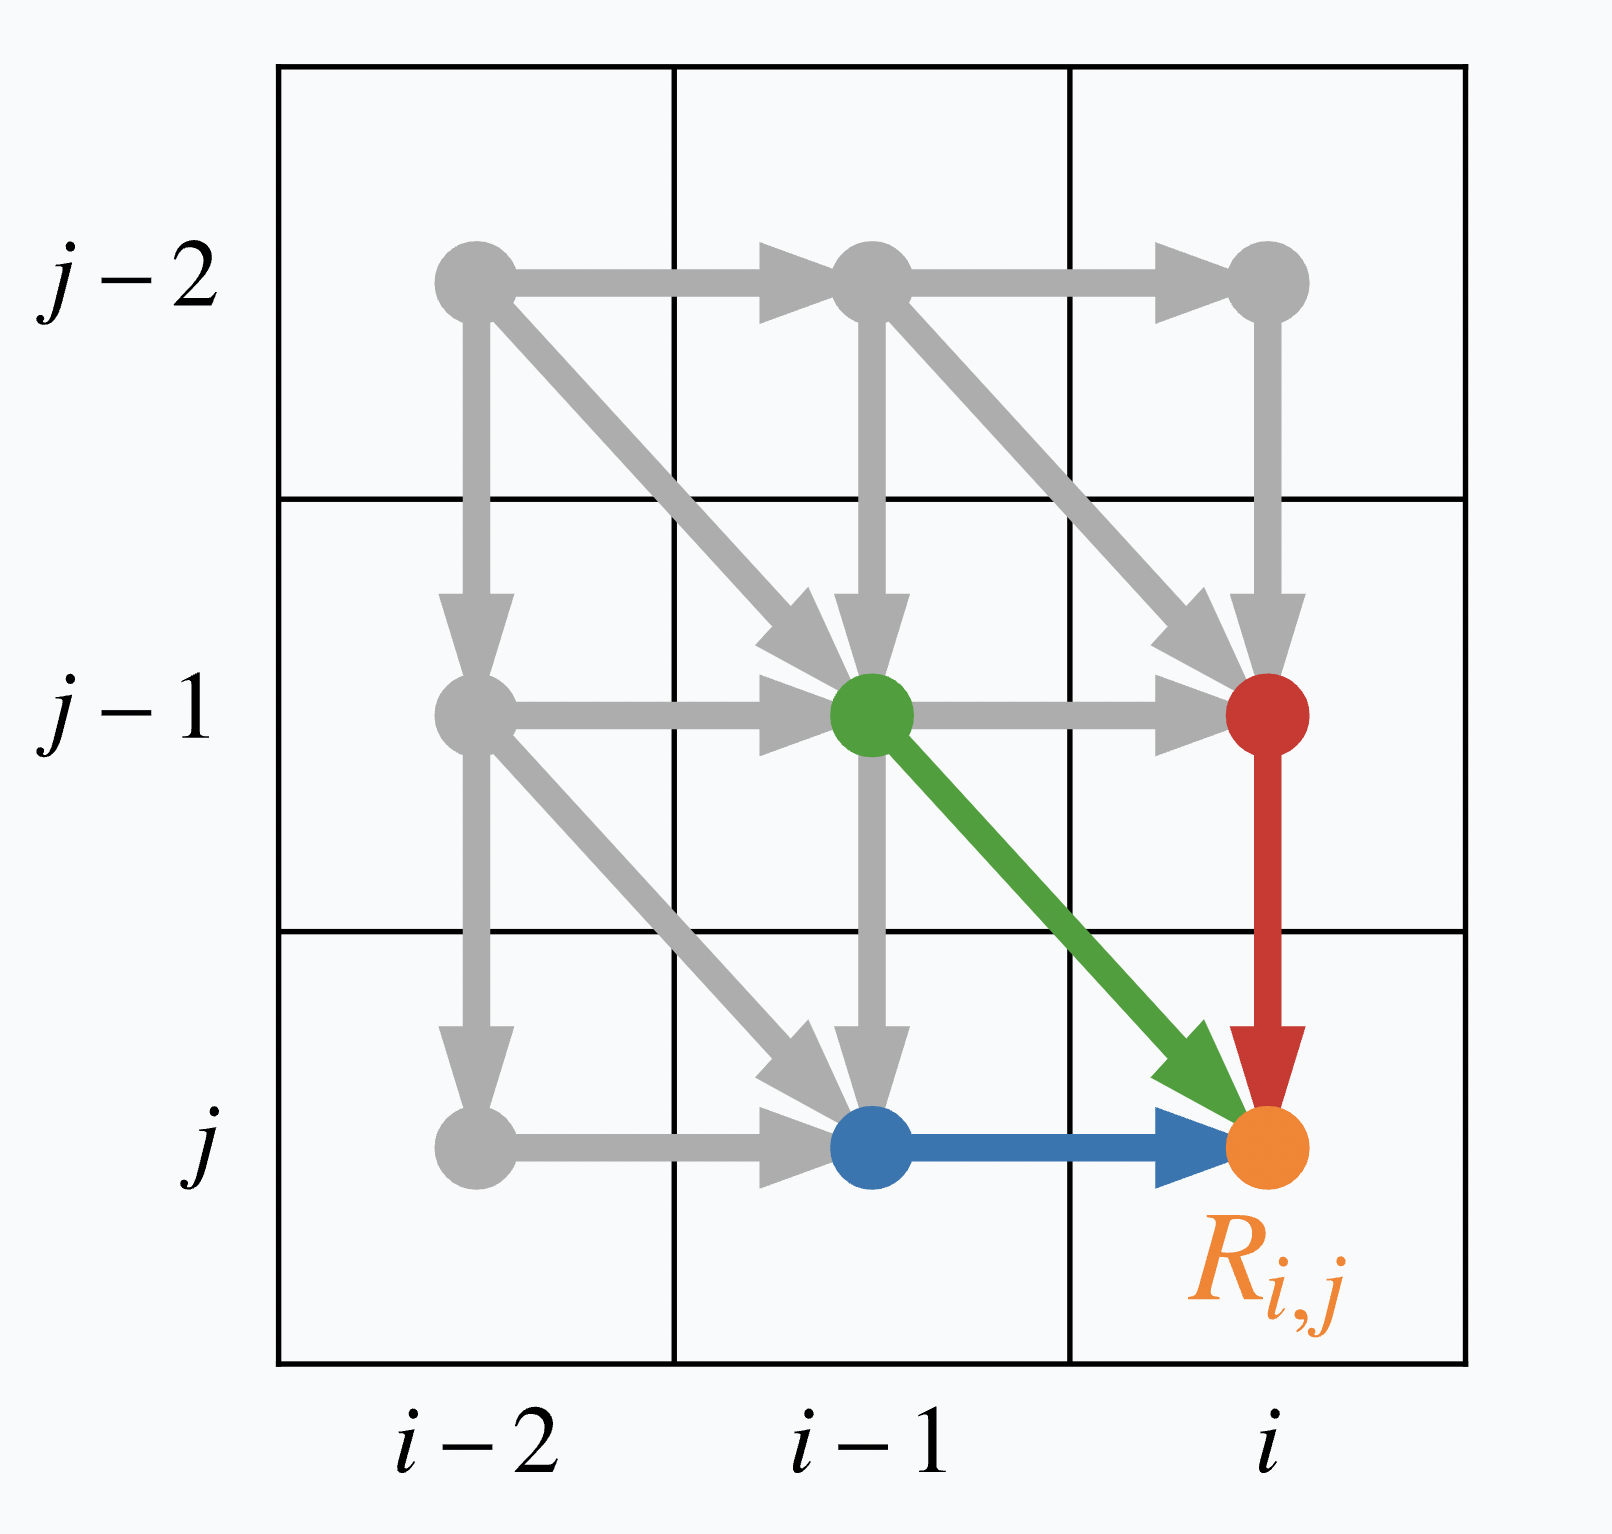
\includegraphics[width=0.8\textwidth]{lecture_7/figs/dtw_transitions.png}
\end{figure}
\end{frame}
%=======
\begin{frame}{DTW Barycenter Averaging}
\textbf{DTW Barycenter Averaging} (DBA) -- это алгоритм, позволяющий найти усреднённый временной ряд в смысле функции расстояния DTW. \\
Алгоритм заключается в итеративном обновлении начального приближения для усреднённого ряда $\hat{x}$ множества временных рядов $x^1, ... x^n$. Одна итерация алгоритма:
\begin{enumerate}
    \item Рассчитаем DTW между $\hat{x}$ и всеми рядами $x^1, .., x^n$.
    \item В результате расчётов мы получим, помимо самих значений DTW, набор выравниваний $\pi_1, ..., \pi_n$ между усреднённым рядом и всеми остальными. Для каждого значения $\hat{x}_i$ найдём множество значений всех остальных рядов, которые попали с данным в пару в одном из выравниваний. Назовём это множество $assoc(\hat{x}_i)$
    \item Обновим каждое значение усреднённого ряда как среднее всех значений других рядов, с которыми данное значение ассоциировано:
    $$ \hat{x}_i := average(assoc(\hat{x}_i)) $$
\end{enumerate}

\end{frame}
%=======

\begin{frame}{DTW Barycenter Averaging, иллюстрация}
\hfill
\begin{figure}[H]
\centering
     \begin{subfigure}[t]{0.45\textwidth}
         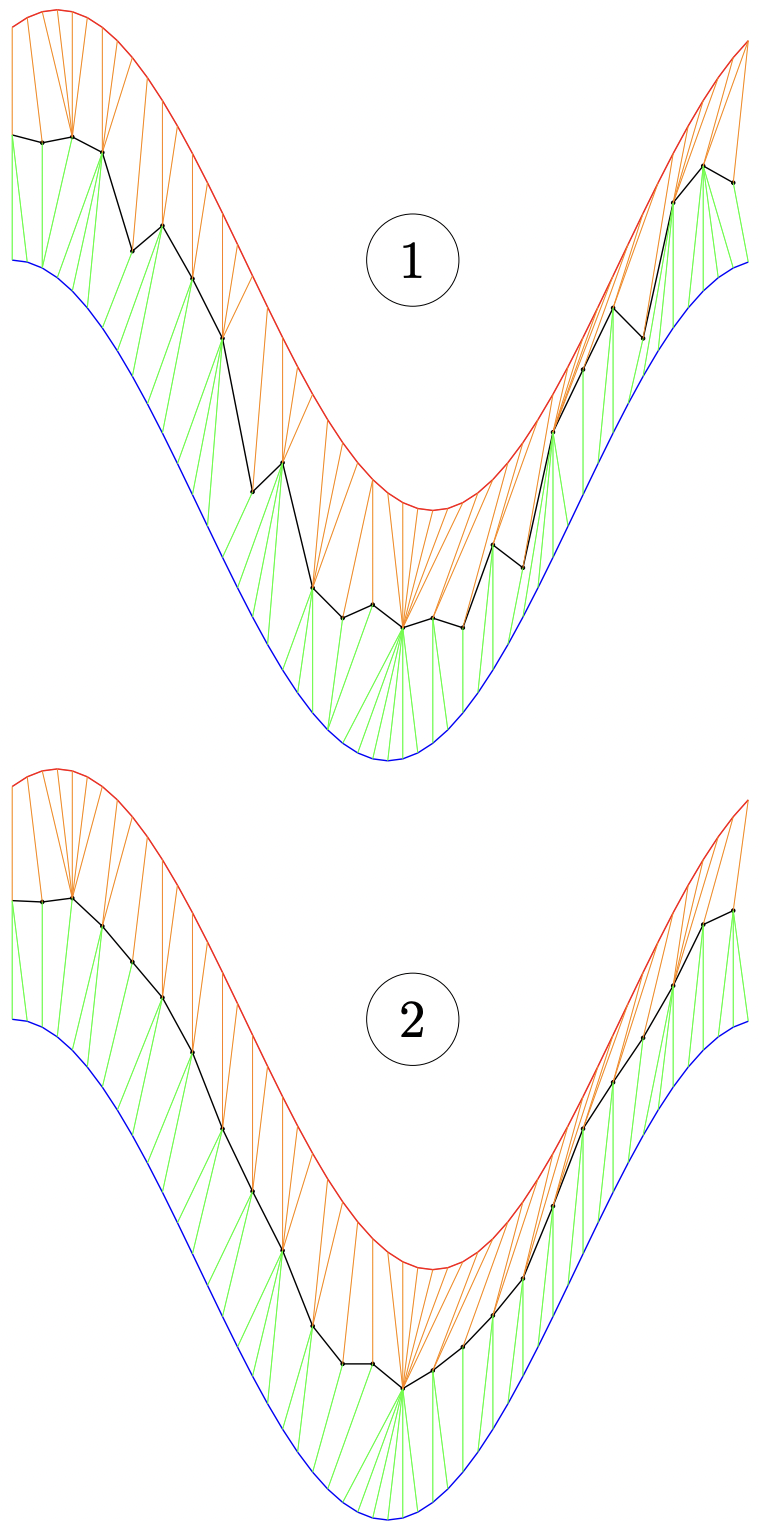
\includegraphics[width=0.7\textwidth]{lecture_7/figs/DBA_1_2.png}
     \end{subfigure}
     \begin{subfigure}[t]{0.45\textwidth}
         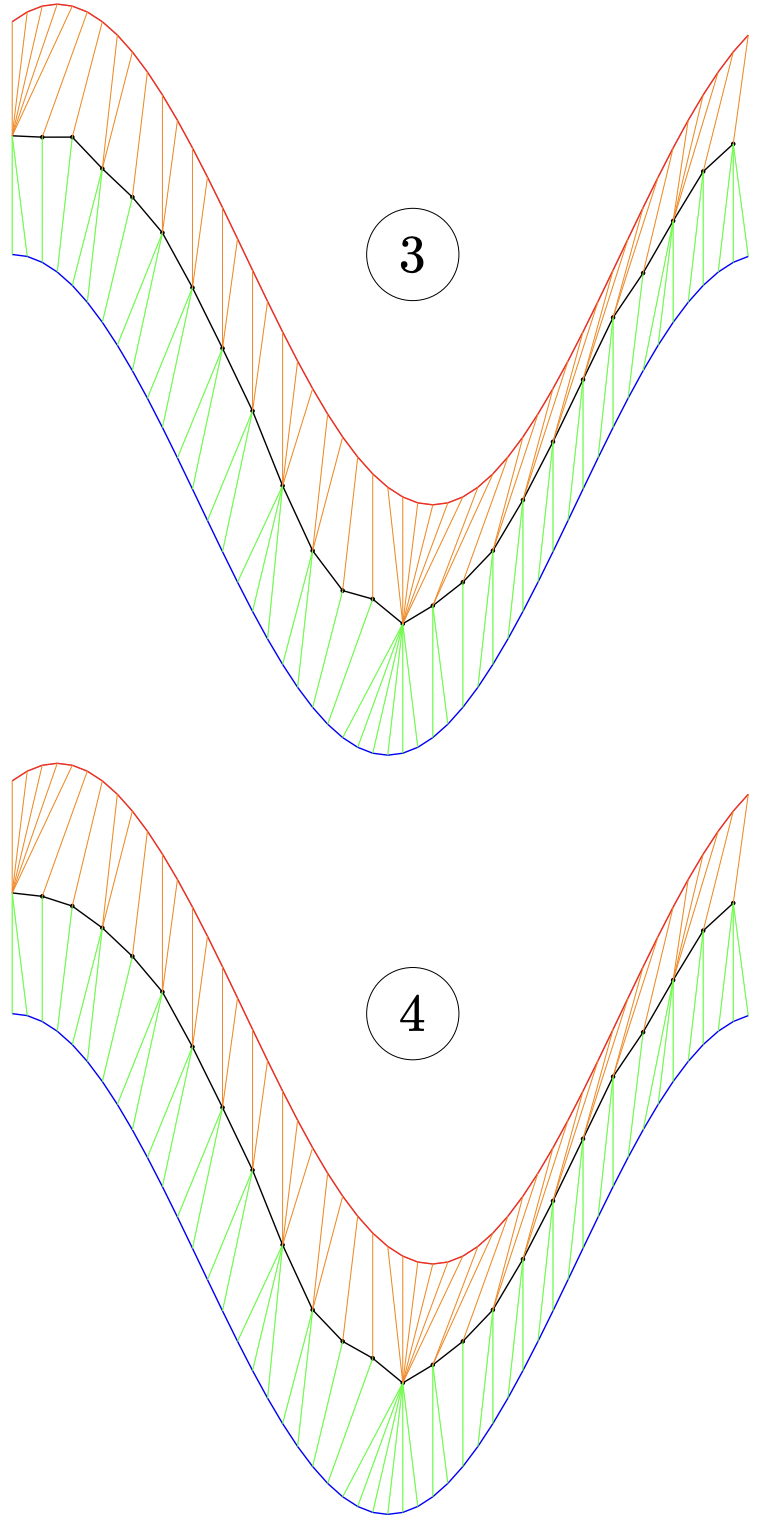
\includegraphics[width=0.7\textwidth]{lecture_7/figs/DBA_3_4.png}
     \end{subfigure}
\end{figure}    
\myfootnotewithlink{https://www.researchgate.net/publication/220601732_A_global_averaging_method_for_dynamic_time_warping_with_applications_to_clustering}{сredit: Petitjean et al. A global averaging method for dynamic time warping, with applications to clustering.} 
\end{frame}
%=======
\begin{frame}{Резюме}
\begin{itemize}
    \item Метод SSA позволяет получать прогноз на одно значение в будущее и с помощью итеративного пересчета увеличивать горизонт предсказания. 
    \item Dynamic time warping -- функция расстояния, позволяющая оценивать поэлементную близость временных рядов с точностью до сдвига/растяжения во времени.
    \item DTW Barycenter Averaging -- удобный способ усреднения временных рядов с учетом их временных сдвигов.
\end{itemize}
\end{frame}
\end{document} 